\documentclass[twocolumn]{article}
\usepackage{graphicx}
\usepackage{amsmath}
\begin{document}
\title{Error function}
\author{Wikipedia, the free encyclopedia}
\date{}
\maketitle

\begin{abstract}
A description of the errorfunction. Made by Wikipedia.
\end{abstract}

\section{Introduction}
In mathematics, the \textbf{error function} (also called the \textbf{Gauss error function}) is a special function (non-Elementary function) of Sigmoid function shape that occurs in probability, statistics, and partial differential equations describing diffusion. It is defined as:


\begin{align}
\mathrm{erf}(x) & = \frac{1}{\sqrt{\pi}}\int_{-x}^x e^{-t^2} dt \\
& = \frac{2}{\sqrt{\pi}}\int_0^x e^{-t^2} dt.
\end{align} 


In statistics, for nonnegative values of $x$, the error function has the following interpretation: for a random variable $Y$ that is normally distributed with mean $0$ and variance $0.5$, erf($x$) describes the probability of $y$ falling in the range [$-x$,$x$].


\begin{figure}
% GNUPLOT: LaTeX picture with Postscript
\begingroup
  \makeatletter
  \providecommand\color[2][]{%
    \GenericError{(gnuplot) \space\space\space\@spaces}{%
      Package color not loaded in conjunction with
      terminal option `colourtext'%
    }{See the gnuplot documentation for explanation.%
    }{Either use 'blacktext' in gnuplot or load the package
      color.sty in LaTeX.}%
    \renewcommand\color[2][]{}%
  }%
  \providecommand\includegraphics[2][]{%
    \GenericError{(gnuplot) \space\space\space\@spaces}{%
      Package graphicx or graphics not loaded%
    }{See the gnuplot documentation for explanation.%
    }{The gnuplot epslatex terminal needs graphicx.sty or graphics.sty.}%
    \renewcommand\includegraphics[2][]{}%
  }%
  \providecommand\rotatebox[2]{#2}%
  \@ifundefined{ifGPcolor}{%
    \newif\ifGPcolor
    \GPcolortrue
  }{}%
  \@ifundefined{ifGPblacktext}{%
    \newif\ifGPblacktext
    \GPblacktexttrue
  }{}%
  % define a \g@addto@macro without @ in the name:
  \let\gplgaddtomacro\g@addto@macro
  % define empty templates for all commands taking text:
  \gdef\gplbacktext{}%
  \gdef\gplfronttext{}%
  \makeatother
  \ifGPblacktext
    % no textcolor at all
    \def\colorrgb#1{}%
    \def\colorgray#1{}%
  \else
    % gray or color?
    \ifGPcolor
      \def\colorrgb#1{\color[rgb]{#1}}%
      \def\colorgray#1{\color[gray]{#1}}%
      \expandafter\def\csname LTw\endcsname{\color{white}}%
      \expandafter\def\csname LTb\endcsname{\color{black}}%
      \expandafter\def\csname LTa\endcsname{\color{black}}%
      \expandafter\def\csname LT0\endcsname{\color[rgb]{1,0,0}}%
      \expandafter\def\csname LT1\endcsname{\color[rgb]{0,1,0}}%
      \expandafter\def\csname LT2\endcsname{\color[rgb]{0,0,1}}%
      \expandafter\def\csname LT3\endcsname{\color[rgb]{1,0,1}}%
      \expandafter\def\csname LT4\endcsname{\color[rgb]{0,1,1}}%
      \expandafter\def\csname LT5\endcsname{\color[rgb]{1,1,0}}%
      \expandafter\def\csname LT6\endcsname{\color[rgb]{0,0,0}}%
      \expandafter\def\csname LT7\endcsname{\color[rgb]{1,0.3,0}}%
      \expandafter\def\csname LT8\endcsname{\color[rgb]{0.5,0.5,0.5}}%
    \else
      % gray
      \def\colorrgb#1{\color{black}}%
      \def\colorgray#1{\color[gray]{#1}}%
      \expandafter\def\csname LTw\endcsname{\color{white}}%
      \expandafter\def\csname LTb\endcsname{\color{black}}%
      \expandafter\def\csname LTa\endcsname{\color{black}}%
      \expandafter\def\csname LT0\endcsname{\color{black}}%
      \expandafter\def\csname LT1\endcsname{\color{black}}%
      \expandafter\def\csname LT2\endcsname{\color{black}}%
      \expandafter\def\csname LT3\endcsname{\color{black}}%
      \expandafter\def\csname LT4\endcsname{\color{black}}%
      \expandafter\def\csname LT5\endcsname{\color{black}}%
      \expandafter\def\csname LT6\endcsname{\color{black}}%
      \expandafter\def\csname LT7\endcsname{\color{black}}%
      \expandafter\def\csname LT8\endcsname{\color{black}}%
    \fi
  \fi
    \setlength{\unitlength}{0.0500bp}%
    \ifx\gptboxheight\undefined%
      \newlength{\gptboxheight}%
      \newlength{\gptboxwidth}%
      \newsavebox{\gptboxtext}%
    \fi%
    \setlength{\fboxrule}{0.5pt}%
    \setlength{\fboxsep}{1pt}%
\begin{picture}(4320.00,3456.00)%
    \gplgaddtomacro\gplbacktext{%
      \csname LTb\endcsname%%
      \put(645,669){\makebox(0,0)[r]{\strut{}$0$}}%
      \csname LTb\endcsname%%
      \put(645,994){\makebox(0,0)[r]{\strut{}$100$}}%
      \csname LTb\endcsname%%
      \put(645,1319){\makebox(0,0)[r]{\strut{}$200$}}%
      \csname LTb\endcsname%%
      \put(645,1644){\makebox(0,0)[r]{\strut{}$300$}}%
      \csname LTb\endcsname%%
      \put(645,1969){\makebox(0,0)[r]{\strut{}$400$}}%
      \csname LTb\endcsname%%
      \put(645,2294){\makebox(0,0)[r]{\strut{}$500$}}%
      \csname LTb\endcsname%%
      \put(645,2619){\makebox(0,0)[r]{\strut{}$600$}}%
      \csname LTb\endcsname%%
      \put(645,2944){\makebox(0,0)[r]{\strut{}$700$}}%
      \csname LTb\endcsname%%
      \put(645,3269){\makebox(0,0)[r]{\strut{}$800$}}%
      \csname LTb\endcsname%%
      \put(821,409){\makebox(0,0){\strut{}$0$}}%
      \csname LTb\endcsname%%
      \put(1341,409){\makebox(0,0){\strut{}$5$}}%
      \csname LTb\endcsname%%
      \put(1860,409){\makebox(0,0){\strut{}$10$}}%
      \csname LTb\endcsname%%
      \put(2380,409){\makebox(0,0){\strut{}$15$}}%
      \csname LTb\endcsname%%
      \put(2900,409){\makebox(0,0){\strut{}$20$}}%
      \csname LTb\endcsname%%
      \put(3419,409){\makebox(0,0){\strut{}$25$}}%
      \csname LTb\endcsname%%
      \put(3939,409){\makebox(0,0){\strut{}$30$}}%
    }%
    \gplgaddtomacro\gplfronttext{%
      \csname LTb\endcsname%%
      \put(153,1969){\rotatebox{-270}{\makebox(0,0){\strut{}Number of Iterations}}}%
      \csname LTb\endcsname%%
      \put(2380,130){\makebox(0,0){\strut{}Matrix Dimension "n"}}%
      \csname LTb\endcsname%%
      \put(3065,3102){\makebox(0,0)[r]{\strut{}Power Iter.}}%
      \csname LTb\endcsname%%
      \put(3065,2916){\makebox(0,0)[r]{\strut{}Inverse Power Iter.}}%
      \csname LTb\endcsname%%
      \put(3065,2730){\makebox(0,0)[r]{\strut{}Shifted Inverse Iter.}}%
      \csname LTb\endcsname%%
      \put(3065,2544){\makebox(0,0)[r]{\strut{}Inverse Iter.}}%
    }%
    \gplbacktext
    \put(0,0){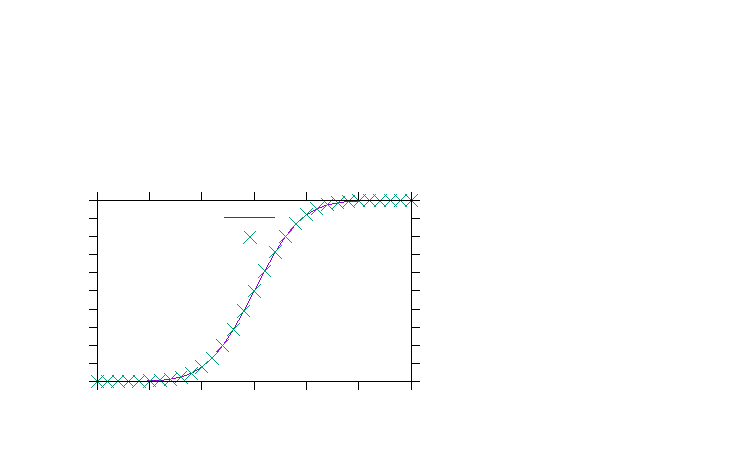
\includegraphics{plot-cairo}}%
    \gplfronttext
  \end{picture}%
\endgroup

\caption{Comparison between the calculated error function using differential equation found in "myerr.c" and the error function from the GSL-library.}
\label{fig-error}
\end{figure}


There are several closely related functions, such as the complementary error function, the imaginary error function, and others.


\section{Name}


The name "error function" and its abbreviation $erf$ were proposed by J. W. L. Glaisher in 1871 on account of its connection with "the theory of Probability, and notably the theory of Errors". The error function complement was also discussed by Glaisher in a separate publication in the same year. For the "law of facility" of errors whose density is given by $f(x)=\left(\frac{c}{\pi}\right)^{\frac{1}{2}}e^{-cx^2}$ (the normal distribution), Glaisher calculates the chance of an error lying between $p$ and $q$ as:
\begin{equation}
\left(\frac{c}{\pi}\right)^{\frac{1}{2}} \int_p^qe^{-cx^2}dx =\frac{1}{2}\left(\mathrm{erf} (q\sqrt{c}) -\mathrm{erf} (p\sqrt{c})\right)\mathrm{.}
\end{equation}

\section{Applications}

When the results of a series of measurements are described by a  normal distribution with standard deviation  $\sigma$ and expected value $0$, then $\mathrm{erf}\left(\frac{a}{\sigma \sqrt{2}}\right)$  is the probability that the error of a single measurement lies between $-a$ and $+a$, for positive $a$. This is useful, for example, in determining the bit error rate of a digital communication system.

The error and complementary error functions occur, for example, in solutions of the heat equation when boundary conditions are given by the Heaviside step function.

The error function and its approximations can be used to estimate results that hold with high probability. Given random variable $X \sim \mathrm{Norm}[\mu,\sigma]$ and constant $L<\mu$:
\begin{equation}
\mathrm{Pr}[X\leq L] = \frac{1}{2} + \frac{1}{2}\mathrm{erf}\left(\frac{L-\mu}{\sqrt{2}\sigma}\right) \approx A \exp \left(-B \left(\frac{L-\mu}{\sigma}\right)^2\right)
\end{equation}

where $A$ and $B$ are certain numeric constants. If $L$ is sufficiently far from the mean, i.e.   $\mu -L \geq \sigma\sqrt{\ln{k}}$, then:

\begin{equation}
\mathrm{Pr}[X\leq L] \leq A \exp (-B \ln{k}) = \frac{A}{k^B}
\end{equation}

so the probability goes to 0 as $k\rightarrow \infty$.


\end{document}
